\documentclass[10pt]{article}

\addtolength{\oddsidemargin}{-.875in}
\addtolength{\evensidemargin}{-.875in}
\addtolength{\textwidth}{1.75in}

\addtolength{\topmargin}{-.875in}
\addtolength{\textheight}{1.75in}

\openup 1em

%macro for commenting
\usepackage{color}
\newcommand{\leo}[1]{{\color{blue}{Leo: #1}}}

% \newcommand{\Xbeta}{ X_i \theta}
\newcommand{\xbeta}{ x_i \beta}
\newcommand{\xtheta}{ x_i \theta}
% \newcommand{\xbetaij}{ x_{ij}^T \theta}
\newcommand{\sgamma}{s_{ij}^T\gamma_i}

\usepackage[round]{natbib}

\usepackage{rotating}
\usepackage{graphicx}
\usepackage{subcaption}

\usepackage{float}
\usepackage{bbm}

\usepackage{amsthm,amsmath, amssymb} 
\usepackage{mathrsfs}
\usepackage{subcaption}
\usepackage{nicefrac}

\usepackage{xcolor}
\newcommand{\aki}[1]{\textcolor{red}{Aki: #1}}

\newtheorem{theorem}{Theorem}
\newtheorem{lemma}{Lemma}
\newtheorem{corollary}{Corollary}
\newtheorem{remark}{Remark}
\newtheorem{example}{Example}


\usepackage{algorithm}
\usepackage{algpseudocode}

%\usepackage{mhequ}
\newcommand{\be}{\begin{equation}\begin{aligned}}
\newcommand{\ee}{\end{aligned}\end{equation}}
\newcommand{\bb}[1]{\mathbb{#1}}
\newcommand{\mc}[1]{\mathcal{#1}}
\DeclareMathOperator{\Binom}{Binomial}
\DeclareMathOperator{\No}{No}
\DeclareMathOperator{\PG}{PG}
\DeclareMathOperator{\IG}{Inverse-Gamma}
\DeclareMathOperator{\Ga}{Gamma}
\DeclareMathOperator{\Bern}{Bernoulli}
\DeclareMathOperator{\U}{Uniform}
\DeclareMathOperator{\Poi}{Poisson}
\DeclareMathOperator{\NB}{NB}
\DeclareMathOperator{\cov}{cov}
\DeclareMathOperator{\var}{var}
\DeclareMathOperator{\diag}{diag}
\DeclareMathOperator{\Diag}{Diag}
\newcommand{\KL}[2]{\textnormal{KL}\left(#1 \parallel #2\right)}
\DeclareMathOperator{\1}{\mathbbm{1}}
\DeclareMathOperator{\bigO}{\mc O}
\newcommand{\dt}{\epsilon} % Stepsize of leapfrog
\newcommand{\mass}{M} % Mass matrix
\newcommand{\hess}{\mathbf{H}} % Hessian notation.



\thispagestyle{empty}
\baselineskip=28pt

\title{\textbf{Extrinsic Priors for Bayesian Modeling with Parameter Constraints}}
\author{Leo Duan, Akihiko Nishimura, David Dunson}
\date{}
\begin{document}
\maketitle
{\bf Abstract:} Prior information often takes for the form of parameter constraints. Bayesian methods include such information through prior distributions having constrained support. By using posterior sampling algorithms, one can quantify uncertainty without relying on asymptotic approximations. However, outside of narrow settings, parameter contraints make it difficult to develop efficient posterior sampling algorithms. We propose a general solution, which relaxes the constraint through the use of an {\em extrinsic prior}, which is concentrated close to the constrained space. General off the shelf posterior sampling algorithms, such as Hamiltonian Monte Carlo (HMC), can then be used directly. We illustrate this approach through multiple examples involving equality and inequality constraints. While existing methods tend to rely on conjugate families, our proposed approach frees us up to define new classes of hierarchical models for constrained problems. We illustrate this through application to a variety of simulated and real datasets.
\vskip 12pt
%\baselineskip=12pt
%\par\vfill\noindent
{\noindent KEY WORDS: Constraint relaxation; Euclidean Embedding; Monotone Dirichlet; Soft Constraint; Stiefel Manifold; Projected Markov chain}
%\par\medskip\noindent
%\clearpage\pagebreak\newpage
\pagenumbering{arabic}


\section{Introduction}
It is extremely common to have prior information available on parameter contraints in statistical models. For example, one may have prior knowledge that a vector of parameters lies on the probability simplex or satisfies a particular set of inequality constraints. Other common examples include shape constraints on functions, positive semidefiniteness of matrices and orthogonality. There is a very rich literature on optimization subject to parameter contraints. One common approach is to rely on Langrange and Karush-Kuhn-Tucker multipliers \citep{boyd2004convex}. However, simply producing a point estimate is often insufficient, as uncertainty quantification (UQ) is a key component of most statistical analyses. Usual large sample asymptotic theory, for example showing asymptotic normality of statistical estimators, tends to break down in constrained inference problems. Instead, limiting distributions may have a complex form that needs to be rederived for each new type of constraint, and may be intractable. An appealing alternative is to rely on Bayesian methods for UQ, including the constraint through a prior distribution having restricted support, and then applying Markov chain Monte Carlo (MCMC) to avoid the need for large sample approximations.

Conceptually MCMC can be applied in a broad class of constrained parameter problems without complications \citep{gelfand1992bayesian}. %\aki{I think sampling from a constrained space, say a manifold, can be challenging even without the computational efficiency issues?}
However, in practice, a primary difficulty is designing a Markov transition kernel that leads to an MCMC algorithm with sufficient computational efficiency to be practically useful. Common default transition kernels correspond to Gibbs sampling, random walk Metropolis-Hastings, and (more recently) Hamiltonian Monte Carlo (HMC). Gibbs sampling relies on alternately sampling from the full conditional posterior distributions for the different parameters, ideally in blocks to improve mixing. Gibbs requires the conditional distributions to be available in a form that is tractable to sample from directly, limiting consideration to specialized models. In constrained problems, block updating is typically either not possible or very inefficient (e.g. relying on rejection sampling with a high rejection probability), and one-at-a-time updating can lead to extremely slow mixing. Random walk algorithms provide an alternative, but each step of the random walk must maintain the parameter constraint. A common approach is to apply a normal random walk and simply reject proposals that violate the constraint, but this can have very high rejection rates even if using an adaptive approach that learns the covariance based on the history of the chain. An alternative is to rely on HMC. In simple settings in which a reparameterization can be applied to remove the constraint, HMC can be applied easily. Otherwise, HMC will generate proposals that violate the constraint, and hence face problems with high rejection rates in heavily constrained problems.

Due to the above hurdles, most of the focus in the literature has been on customized solutions developed for specific constraints.
One popular strategy is to carefully pick a prior and likelihood such that posterior sampling is tractable. For example, for modeling of data on manifolds, it is typical to restrict attention to specific models, such as the Bingham-von Mises-Fisher distribution for Stiefel manifolds \citep{khatri1977mises,hoff2009simulation}. For data on the probability simplex, one instead relies on the Dirichlet distribution. An alternative is to reparameterize the model to eliminate or simplify the constraint. For example, when faced with a monotonicity constraint, one may reparameterize in terms of differences as the resulting positivity constraint leads to much easier sampling (REFs). In the literature on modeling of data on manifolds, there are two strategies: (i) {\em intrinsic} methods that define a statistical model directly on the manifold, and (ii) {\em extrinsic} methods that indirectly induce a model on the manifold through embedding the manifold in a Euclidean space, defining a model in the Euclidean space, and then projecting back onto the manifold. Essentially all of the current strategies for Bayesian modeling with constraints take an intrinsic-style approach. However, by strictly maintaining the constraint at all stages of the modeling and computation process, one limits the possibilities in terms of defining general methods to deal with parameter constraints.

These drawbacks motivate the development of {\em extrinsic} approaches that define an unconstrained model and/or computational algorithm, and then somehow adjust for the constraint. A related idea is \cite{gelfand1992bayesian}, who suggested running Gibbs sampling ignoring the constraint but only accepting the draws satisfying the constraint. Unfortunately, such an approach is highly inefficient, as motivated above. An alternative is to run MCMC ignoring the constraint, and then project draws from the unconstrained posterior to the appropriately constrained space. Such an approach was proposed for generalized linear models with order constraints by \cite{dunson2003bayesian}, extended to functional data with monotone or unimodal constraints \cite{gunn2005transformation}, and recently modified to nonparametric regression with monotonicity \cite{lin2014monogp} or manifold \cite{lin2016extrinsic} constraints.

An alternative idea is to {\em relax} a sharp parameter constraint by defining a prior that has unrestricted support but places small probability outside of the constrained region. \cite{neal2011mcmc} suggested such an approach to apply HMC in settings involving a simple truncation constraint, while \cite{pakman2014exact} applied a related idea to improve sampling from truncated multivariate normal distributions.

The goal of this article is to dramatically generalize these specific approaches to develop a broad class of {\em extrinsic priors} for parameter constrained problems. These priors are defined to place small probability outside of the constrained region, while permitting use of efficient and general use MCMC algorithms; in particular, HMC. When the constraints need to upheld strictly, the approximation can be corrected with a simple projection, followed by a Metropolis-Hastings step with high acceptance probability.
Unlike intrinsic methods, such as Riemannian and geodesic HMC \citep{girolami2011riemann,byrne2013geodesic}, our approach is
relatively efficient and simple to implement in general settings using automatic algorithms. The generality frees up a much broader spectrum of Bayesian models, as one no longer needs to focus on very specific computationally tractable models.
Theoretic studies are conducted and original models are shown in simulations and data applications.

\section{Extrinsic Bayes Methodology}


\subsection{Conditioned Intrinsic Distribution}

Let $\theta \in \mc D$ denote the parameters in likelihood function $L(\theta;y)$, with $y$ the data. The support $\mc D$ is a constrained space. The usual Bayesian approach assigns a prior density $\pi_{0,\mc D}(\theta)$ for $\theta$ having support $\mc D$. Traditional strategy is to reparameterize $\theta$ with $f(\theta)$ to always satisfy $\theta \in \mc D$, and find an {\it intrinsic} distribution on $\mc D$. \cite{diaconis2013manifold} provide a detailed review on these methods. Although some of them are successful, in general, reparameterization does not always exist and achieving desired property (such as uniformity on $\mc D$) can be difficult due to variable transformation.

We now present a different intrinsic strategy that does not involve transformation. Assuming that $\mc D \subset \mc R$, with $\mc R$ denoting a `less constrained' space, we start with an unconstrained prior $\pi_{0,\mc R}(\theta)$, conditioning it on a random variable $\omega=\mathbbm{1}_{\theta\in \mc D}$ to obtain conditional density $\pi_{0,\mc D}(\theta)= \pi_{0,\mc R}(\theta \mid \omega=1)$. We call this `conditioned intrinsic distribution'. In order to utilize the various existing distribution families and geometric measure thoery, we focus on $\mc R$ being Eucledean space $\mathbb{R}^{p}$ or its truncated subspace.

Let $(\Omega, \mathscr B, P)$ be a probability space and sub-$\sigma$-field $\mathscr A\subseteq \mathscr B$, the function $P(\cdot\mid \mathscr A)$ is a {\it regular conditional probability} (r.c.p.) \citep{kolmogorov1950foundations} on $\mathscr B$ given $\mathscr A$, if:
\begin{enumerate}
	\item For each $\omega\in  \Omega$, $P(\cdot\mid \mathscr A)(\omega)$ is a probability measure on $\mathscr B$.
	\item For each $B\in \mathscr B$, the mapping $P(B\mid \mathscr A)(.)$ is $\mathscr A$- measurable.
	\item For each $A \in \mathscr A$, $B\in \mathscr B$, $P(A\cap B)=\int_{A} P(B\mid \mathscr A)(\omega)P(d\omega)$.
\end{enumerate}

In our case, recall $\omega=1$ if $\theta\in \mc D$ and equal $0$ otherwise. Let $Z(\mc D)=\int_{\mc D} \pi_{0,\mc R}(\theta)d\theta \in [0,1)$, we first assign:

\begin{equation}
\label{rcp}
	P(\omega) = w Z(\mc D)  + (1-w)(1-Z(\mc D)), \qquad  P(B \mid  \mathscr A)(\omega)={P({B\cap  \mc D} \mid \omega=1)} \omega +  {P({B\cap (\mc R \setminus \mc D})\mid \omega=0)}(1-\omega),
\end{equation}
where $P({B\cap (\mc R \setminus \mc D})\mid \omega=0)$ is a probability measure that we are not interested in; rather, our focus is on ${P({B\cap  \mc D} \mid \omega=1)}$. When $Z(\mc D)>0$, one can simply define:

\begin{equation}
\begin{aligned}
\label{exact_prior1}
 \int_{B} \pi_{0,\mc D}(\theta) d\theta= {P({B\cap  \mc D} \mid \omega=1)}=\int_{B} \frac{  \pi_{0,\mc R}(\theta) \mathbbm{1}_{\theta\in \mc D}}{ Z(\mc D) } d\theta  .
\end{aligned}
\end{equation}

When $Z(\mc D)=0$, in \eqref{rcp}, any proper ${P({B\cap  \mc D} \mid \omega=1)}$ would satisfy the r.c.p criteria. However, one can still utilize $\pi_{0,\mc R}(\theta)$ by considering measure at a lower dimension $m<n$. As an intuitive example, a surface can have Lebesgue volume $\lambda^3(\mc D)=0$, but positive area on a 2-dimensional manifold.

Formally, for a set $\mc D$, if it is the Lipschitz image of a bounded subset in $\mathbb R^m$ (known as `$m$-rectifiable'), it has Minkowski content \citep{federer2014geometric}:

\begin{equation}
\label{minkowski}
	\mc M^m(\mc D)=\lim_{r\rightarrow 0_+}\frac{\lambda^n(\mc D_r)}{\alpha_{n-m} r^{n-m}}
\end{equation}
where $\alpha_t=\frac{\Gamma(\frac{1}{2})^{t}}{\Gamma(1+ \frac{t}{2})}$, with $\mc D_r=\{x\in \mathbb{R}^n: \text{dist}(x,y)<r, y\in \mc D\}$ known as the open r-parallel set, $\text{dist}(.,.)$ is a distance; $\lambda^n(\mc D_r)={ \int_{\mc D_r} \pi_{0,\mc R}(\theta)}d\theta$ is its Lebesgue measure in $\mathbb{R}^n$. Due to the expansion, $\lambda^n(\mc D_r)>0$ for $r>0$.

%Clearly, when $m=n$,  $\mc M^m(\mc D)=0$ if $\lambda^n(\mc D)=0$; when $m=0$, this reduces to counting measure. $\text{dim}_{\mc M}(\mc D)=\inf\{t; \mc M^t(\mc D)=0\}=\sup\{t; \mc M^t(\mc D)=\infty\}$ is called the Minkowski dimension.

When $m$ is chosen such that $0<\mc M^m(\mc D)<\infty$, then one calls $\mc D$ $m$-dimensional Minkowski measurable, and $\mc M^m(\mc D)$ is proportional to the Hausdorff measure $\mc H^{m}(\mc D)$ for $m$-rectifiable $\mc D$ \citep{federer2014geometric}. Finding the appropriate $m$ can be challenging; however, we do not need $m$ for the relative measure between $B\cap  \mc D$ and $\mc D$.
Letting $P({B\cap  \mc D} \mid \omega=1)\propto \mc M^m(B\cap\mc D)$ and $P({\mc D} \mid \omega=1)=1$ yields:

\begin{equation}
\label{exact_prior2}
	\int_{B} \pi_{0,\mc D}(\theta) d\theta= P({B\cap  \mc D} \mid \omega=1)= \frac{\mc M^m(\mc B\cap \mc D)}{\mc M^m(\mc D)}= \lim_{r\rightarrow 0_+}\frac{\lambda^n(B\cap \mc D_r)}{\lambda^n(\mc D_r)} 
=\lim_{r\rightarrow 0^+} \frac{\int_{ B} \pi_{0,\mc R}(\theta) \mathbbm{1}_{\theta\in \mc D_r} d\theta}{ \int_{\mc D_r} \pi_{0,\mc R}(\theta)}
\end{equation}
where the terms involving $m$ are canceled, due to $\mc M^m(B\cap\mc D)=\lim_{r\rightarrow 0_+}\frac{\lambda^n(B\cap \mc D_r)}{\alpha_{n-m} r^{n-m}}$ \citep{winter2016localization}. This result is extensible to unbounded set $\mc D$ provided $0<\mc M^m(\mc D)<\infty$ for certain $m$, although the equivalence of Minkowski content and Hausdorff measure may not hold.

Similarly, letting the likelihood function be $L(y;\theta)$, the posterior of $\theta$ is $\pi_{\mc D}(\theta \mid y)=\frac{ L(y;\theta) \pi_{0,\mc D}(\theta)}{{\int_\mc D}L(y;\theta) \pi_{0,\mc D}(\theta)d\theta}$. If $\int_{\mc D} \pi_{0,\mc R}(\theta)d\theta >0$ and $\int_{\mc R} L(y;\theta)\pi_{0,\mc R}(\theta) \mathbbm{1}_{\theta\in \mc D}d\theta >0$,

\begin{equation}
\label{exact_posterior1}
	{\pi}_{\mc D}(\theta \mid y) = \frac{ L(y;\theta)\pi_{0,\mc R}(\theta)\mathbbm{1}_{\theta\in \mc D} }{ \int_{\mc R} L(y;\theta)\pi_{0,\mc R}(\theta) \mathbbm{1}_{\theta\in \mc D}d\theta };
\end{equation}
otherwise,

\begin{equation}
\label{exact_posterior2}
	\int_{B} {\pi}_{\mc D}(\theta \mid y) d\theta = \lim_{r\rightarrow 0^+}  \frac{ \int_{B}  L(y;\theta)\pi_{0,\mc R}(\theta)\mathbbm{1}_{\theta\in \mc D_r}  d\theta }{ \int_{\mc R} L(y;\theta)\pi_{0,\mc R}(\theta) \mathbbm{1}_{\theta\in \mc D_r}d\theta }.
\end{equation}

Therefore, both prior and posterior can be obtained intrinsically via this conditioning approach, although the posterior sampling is generally difficult and \eqref{exact_prior2}\eqref{exact_posterior2} may become intractable.

We now use an example to illustrate this strategy approach when $Z(\mc D)=0$.

{\bf Example 1A: Two Gaussians with Sum Constraint (Conditioned Intrinsic)}

Consider a bivariate Gaussian random vector $[\theta_1,\theta_2]' \sim \No(0,I)$ in constrained space $\mc D=\{(\theta_1,\theta_2):\theta_1+\theta_2=1\}$. Denoting $\phi(x)= \frac{1}{\sqrt{2\pi}} \exp(-\frac{x^2}{2})$, $Z(\mc D)=\int_{\mc D} \phi(\theta_1)\phi(\theta_2)d\theta =0$. Using $\mc D_r=\{(\theta_1,\theta_2):\theta_1+\theta_2 \in (1-r, 1+r)\}$ and $B= \{(\theta_1,\theta_2): \theta_1< x, \theta_2\in \mathbb R\}$,

\begin{equation*}
	\begin{aligned}
\int_{B} \pi_{0,\mc D}(\theta) d\theta= 
& \lim_{r\rightarrow 0^+}\frac{
	\int_{(1-r)}^{(1+r)} \int_{-\infty}^{x} \phi(\theta_1)\phi(z-\theta_1) d\theta_1 dz  
}{
\int_{(1-r)/\sqrt 2}^{(1+r)/\sqrt 2} \phi(z) dz
} \\ 
= & \lim_{r\rightarrow 0^+}\frac{ \frac{\partial}{\partial r}
	\int_{(1-r)}^{(1+r)} \int_{-\infty}^{x} \phi(\theta_1)\phi(z-\theta_1) d\theta_1 dz  
}{
\frac{\partial}{\partial r}\int_{(1-r)/\sqrt 2}^{(1+r)/\sqrt 2} \phi(z) dz
} \\ 
= &  
\lim_{r\rightarrow 0^+}\frac{
	\int_{-\infty}^{x} \phi(\theta_1)\left( \phi({1+r} -\theta_1) d\theta_1  +  \phi({1-r}-\theta_1)\right) d\theta_1  
}{\phi (\frac{1+r}{\sqrt 2})/\sqrt 2 + \phi (\frac{1-r}{\sqrt 2})/\sqrt 2} \\
= & \int_{-\infty}^{x} \frac{\sqrt{2}}{\sqrt{2\pi}} \exp(-\frac{(\theta_1-\frac{1}{2})^2}{2/2}) d\theta_1,
\end{aligned}
\end{equation*}
which corresponds to $\theta_1\mid (\theta_1+ \theta_2=1) \sim \No(1/2,1/2)$, $\theta_2\mid \theta_1 \sim \delta_{1-\theta_1}$ with $\delta_x$ denoting a point mass at $x$. Marginally, this is a degenerate bivariate Gaussian distribution:
$$\begin{bmatrix} \theta_1 \\ \theta_2 \end{bmatrix} \sim
\No_{\text d} \left(
 \begin{bmatrix} \frac{1}{2} \\ \frac{1}{2} \end{bmatrix},
\begin{bmatrix} \frac{1}{2} & -\frac{1}{2}  \\  -\frac{1}{2}  & \frac{1}{2} \end{bmatrix}
\right).$$



\subsection{Extrinsic Bayes}
The conditioned intrinsic distribution relies on the sharp indicator function $\mathbbm{1}_{\theta\in \mc D}$ and limit of open r-parallel set $\mc D_r$, leading to computational difficulty in prior and posterior. We now propose an extrinsic prior that builds on \eqref{exact_prior1} and \eqref{exact_prior2}, approximating $\mathbbm{1}_{\theta\in \mc D}$ with a {\em smooth} alternative $\mc{K}( \theta; \mc D)$ with less contrained support:

\begin{equation}
\label{extrinsic_prior}
	\tilde{\pi}_{0,\mc D}(\theta) = \frac{ \pi_{0,\mc R}(\theta) \mc{K}( \theta; \mc D) }{ \int_{\mc R} \pi_{0,\mc R}(\theta) \mc{K}(\theta; \mc D)d\theta }
\end{equation}
where $\mc K(\theta; \mc D)$ satisfies $\mc K(\theta; \mc D)=1$ if $\theta\in \mc D$ and $ \int_{\mc R} \pi_{0,\mc R}(\theta) \mc{K}(\theta; \mc D)d\theta>0$. When $Z(\mc D)=0$, $\mc K(\theta;  \mc D)=\lim_{r\rightarrow 0^+}\mc K(\theta;  \mc D_r)$ with $\mc{K}(\theta; \mc D_r)$ approximating $\mathbbm{1}_{\theta\in  \mc D_r}$, then $
	\int_{B} \tilde{\pi}_{0,\mc D}(\theta) d \theta =  \lim_{r\rightarrow 0^+}\frac{\int_{B}  \pi_{0,\mc R}(\theta) \mc{K}( \theta; \mc D_r)d\theta }{ \int_{\mc R} \pi_{0,\mc R}(\theta) \mc{K}(\theta; \mc D_r)d\theta } = 	\int_{B} \frac{ \pi_{0,\mc R}(\theta) \mc{K}( \theta; \mc D) }{ \int_{\mc R} \pi_{0,\mc R}(\theta) \mc{K}(\theta; \mc D)d\theta } d\theta$. Therefore, the limit forms in \eqref{exact_prior2} and \eqref{exact_posterior2} are no longer needed. The posterior takes similar form

\begin{equation}
\label{extrinsic_posterior}
	\tilde{\pi}_{\mc D}(\theta \mid y) = \frac{ L(y;\theta)\pi_{0,\mc R}(\theta) \mc{K}( \theta; \mc D) }{ \int_{\mc R} L(y;\theta)\pi_{0,\mc R}(\theta) \mc{K}(\theta; \mc D)d\theta }.
\end{equation}

We now define $\mc K(\theta;\mc D)$. Assuming there are $m$ constraints with each defining a constrained subspace $\mc D_k$, $\mc D = \bigcap_{k=1}^m\mc D_k$, we have

\begin{equation}
\label{smoothing}
\mc K(\theta; \mc D)= \prod_{k=1}^m K_k(v_k(\theta)),
\end{equation}
where $v_k: \mc R \rightarrow [0,\infty)$ is a measurable function and quantifies the distance to space $\mc D_k$. For example, one can use $v(\theta)=|f(\theta)|$ as a distance to equality-constrained space  $\{\theta:f(\theta)=0\}$; $v(\theta)=|f(\theta)|_+$, where $(x)_+ = \left\{\begin{array}{cc}  0 \text{ if } x\le 0 \\ x \text{ if } x> 0\end{array}\right.$ as a distance to inequality-constrained space  $\{\theta:f(\theta) \le 0\}$. The function $K_k:[0,\infty)\rightarrow [0,1]$ penalizes $v_k(\theta)>0$ and decreases in $v_k(\theta)$. For example, $K_k(v)=\exp(-v)$ or $K_k(v)=\frac{1}{1+v^2}$. For illustration simplicity, in this paper, we focus on exponential smoothing function $K_k(v(\theta))=\exp(-\frac{v(\theta)}{\lambda_k})$ with $\lambda_k>0$ as a tuning parameter. We assume that the extrinsic prior is proper $ \int_{\mc R} \pi_{0,\mc R}(\theta) \mc{K}(\theta; \mc D)d\theta <\infty$.


This framework is applicable to a variety of complicated case. For example, $\theta$ can have only some of parameters constrained; parameters can be in multiple constraints simultaneously; constraints can be dependent. Regardless, it is generally simple to adapt \eqref{smoothing} via appropriate mapping through $v(\theta)$. 

We now provide some additional regularity conditions on $v_k$ and $K_k$: for $k=1,\ldots,m$, $v_k(\theta)=0$ only if $\theta\in \mc D_k$ and $K_k(v)=1$ only if $v=0$. Therefore, $\theta\in \mc D$ $\Leftrightarrow$ all $v_k(\theta)=0$ $\Leftrightarrow$ $\mc K(\theta; \mc D)=1$, this ensures $\mc K(\theta; \mc D)$ is the same as the indicator function for $\theta\in \mc D$.

To illustrate, consider a truncated normal prior $\No_{(-\infty,5)}(0,5^2)$. The unnormalized density of intrinsic prior is $\exp(-{\theta^2}/{2\cdot 5^2})\mathbbm{1}_{\theta\in (-\infty,5)}$, which can be approximated by  extrinsic prior $\exp(-{\theta^2}/{2\cdot 5^2}) \exp(-v(\theta))$. We plot two distances $v(\theta)=(\theta-5)_+$ and $v(\theta)=(\theta-5)^2_+$ in Figure~\ref{truncated_normal}. Inside $\mc D=(-\infty,5)$, both intrinsic and extrinsic distribution are the same, except for a different normalizing constant; outside $\mc D$, intrinsic one drops directly to $0$ at the boundary, whereas the extrinsic one decreases smoothly.

\begin{figure}[H]
 \centering
 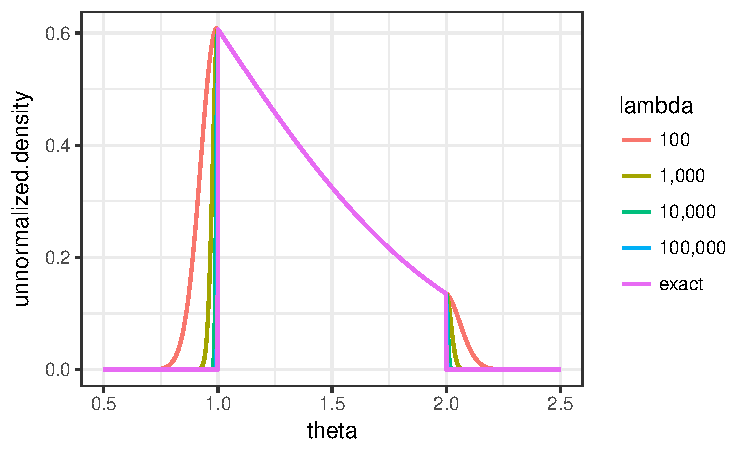
\includegraphics[width=0.5\textwidth]{density_truncated_normal}
\caption{Unnormalized densities for truncated normal $\No_{(-\infty,5)}(0,5^2)$ under exact intrinsic prior and approximating extrinsic prior. Inside $(-\infty,5)$, the priors are the same up to a constant difference. The intrinsic prior abruptly drops to $0$ on the boundary, while the approximating ones drop smoothly. Intrinsic prior based on first-order $v(\theta)$ drops faster than the one based on second order when $v(\theta)\in (0,1)$.}
\label{truncated_normal}
\end{figure}

We now apply extrinsic Bayes in the previous example of two Gaussians under sum constraint.

{\bf Example 1B: Two Gaussians with Sum Constraint (Extrinsic Approach)}

We now use extrinsic prior $\tilde\pi_{0,\mc D}(\theta) \propto \exp(-\frac{\theta_1^2+\theta_2^2}{2})\exp(-\frac{v(\theta)}{\lambda})$. Choosing $v(\theta)= (\theta_1+\theta_2-1)^2$ allows us to obtain closed-form for the extrinsic prior $\theta_1 \sim \No(\frac{2}{\lambda+4},\frac{\lambda+2}{\lambda+4})$, $\theta_2\mid \theta_1 \sim \No(\frac{2}{\lambda+2}(1-\theta_1),\frac{\lambda}{\lambda+2})$. Marginally, 

$$\begin{bmatrix} \theta_1 \\ \theta_2 \end{bmatrix} \sim
\No \left(
 \begin{bmatrix} \frac{2}{\lambda+4} \\ \frac{2}{\lambda+4} \end{bmatrix},
\begin{bmatrix} \frac{\lambda+2}{\lambda+4} & -\frac{2}{\lambda+4}  \\  -\frac{2}{\lambda+4}  &\frac{\lambda+2}{\lambda+4} \end{bmatrix}
\right).$$
As $\lambda\rightarrow 0$, the extrinsic prior becomes the same as the degenerate bivariate Gaussian in intrinsic approach.

Clearly the approximation based on extrinsic approach is much simpler to derive compared to the conditioned intrinsic distribution.

\subsection{Approximation Error}
\leo{We have asymptotic results on total variation distance going to 0, and non-asymptotic bound when $\lambda>m>0$, if  $\int_{\mc D} \pi_{\mc R}(\theta)d\theta>0$. But the non-asymptotic bound fails if  $\int_{\mc D} \pi_{\mc R}(\theta)d\theta=0$. If we are to bound distance between two measures, we might need to switch to Wasserstein distance with Eucledean norm in the whole section.}

We now study the properties of the extrinsic prior and posterior. One important task is to quantify the difference between extrinsic and intrinsic ones. Due to similar reasoning for prior and posterior, we use some general notation. Let $\pi_{\mc R}(\theta)$ be an unnormalized density in $\mc R$, which is $\pi_{0,\mc R}(\theta)$ when studying prior and $L(y;\theta)\pi_{0,\mc R}(\theta)$ when studying posterior; $\Pi(.)$ and $\tilde\Pi(.)$ to represent the measures under intrinsic and extrisic methods associated with either prior or posterior distribution. 

We first explore the case case in \eqref{exact_prior1} and  \eqref{exact_posterior1}, where $\int_{\mc D} \pi_{\mc R}(\theta)d\theta>0$.

%distance between extrinsic and intrinsic
\begin{remark}
Let $M_1= \int_{\mc R} \pi_{0,\mc R}(\theta) \mathbbm{1}_{\theta\in \mc D} d\theta$ and $M_2 = \int_{\mc R} \pi_{\mc R}(\theta) \mc K(\theta;\mc D)d\theta$, when $M_1>0$, the total variation distance between the measures of extrinsic and intrinsic distributions is
$$||\Pi(.), \tilde{\Pi}(.) ||_{TV} = 1 - \frac{M_1}{M_2} \le \frac{\int_{\mc R \setminus \mc D} \pi_{\mc R}(\theta) \mc K(\theta;\mc D)d\theta}{M_1}.$$
\end{remark}
proof:
{Via definition of total variation distance and $\mc K(\theta;\mc D)=1$ when $\theta\in\mc D$.}

Using exponential smoothing function $\mc K(\theta; D) = \prod_{k=1}^m \exp( -v_k(\theta)/\lambda_k)$, as all $\lambda_k \rightarrow 0$, the total variation $||\Pi(.), \tilde{\Pi}(.) ||_{TV} \rightarrow 0$, if $\int_{\mc R} \pi_{\mc R}(\theta) d\theta<\infty$. This is a direct result of dominated convergence theorem and $\mc K(\theta; \mc D)\le 1$.


With some mild assumptions, we further quantify the non-asymptotic rate. Letting $\lambda = \sup_k \lambda_k$, $M= \int_{\mc R \setminus \mc D} \pi_{\mc R}(\theta) d\theta<\infty$. As a linear combination of measurable functions, $v(\theta)=\lambda\sum_{k=1}^m\frac{ v_k(\theta)}{\lambda_k}$ is measurable. Let $f(v)$ be the density of $v(\theta)$.

\begin{remark}
\label{convergence_rate}
If there exists a $t<\infty$ such that $f(v) < \infty$, for any $t>0$,
$$\int_{\mc R \setminus \mc D} {\pi_{\mc R}(\theta)} \prod_{k=1}^m \exp( -v_k(\theta)/\lambda_k) d \theta \le 
 {M} \exp(-\frac{t}{\lambda}) + {M} \sup_{t^*\in(0,t)} {f(t^*)}\lambda 
$$
\end{remark}
\aki{The density of $v(\theta)$ crucially depends on the level set of $v(\theta)$ and is a pretty complicated (i.e.\ intractable) object in general.}

\leo{The point is that if the measure of $v$ is Lipschitz in a $t$-ball of $\mc D$, then $\sup_{t^*\in(0,t)} {f(t^*)}$ is bounded; $\exp(-\frac{t}{\lambda})$ goes to $0$ faster than $\lambda$, so the whole term goes to $0$ in $\mc O(\lambda)$.}

\begin{proof}[Proof]
\begin{equation}
\begin{aligned}
\frac{1}{M}\int_{\mc R \setminus \mc D} {\pi_{\mc R}(\theta)} \prod_{k=1}^m \exp( -v_k(\theta)/\lambda_k) d \theta = & 
\mathbb{E} \exp(- \frac{v}{\lambda}) \\
= & \mathbb{E} \mathbbm{1}_{(0,t)} \exp(- \frac{v}{\lambda}) +  \mathbb{E} \mathbbm{1}_{(t,\infty)} \exp(- \frac{v}{\lambda}) \\
\le & \int_0^t f(v) \exp(- \frac{v}{\lambda}) dv + \exp(-\frac{t}{\lambda}) \\
\le & \sup_{t^*\in(0,t)} f(t^*) \int_0^t \exp(- \frac{v}{\lambda}) dv + \exp(-\frac{t}{\lambda}) \\
= & \sup_{t^*\in(0,t)} f(t^*)  \lambda (1- \exp(-t/\lambda)) + \exp(-\frac{t}{\lambda}) \\
\le  & \sup_{t^*\in(0,t)} f(t^*)  \lambda  + \exp(-\frac{t}{\lambda}) \\
\end{aligned}
\end{equation}
Rearranging terms yields the result.
\end{proof}

For $\lambda$ close to $0$, the extrinsic measure approaches intrinsic one in total varation distance in $O(\lambda)$. This rate is quantified under very general assumption. We expect it can be sharpened under special cases.

We now examine the second case in \eqref{exact_prior2} and \eqref{exact_posterior2} where ${ \int_{\mc D} \pi_{\mc R}(\theta)d\theta }=0$.


\begin{remark}
If both $\lim_{r\rightarrow 0^+} \frac{\int_{B} \pi_{\mc R}(\theta) \mathbbm{1}_{\theta\in \mc D_r} d\theta}{ \int_{\mc D_r} \pi_{\mc R}(\theta)d\theta }$ and $ \lim_{r\rightarrow 0^+}\frac{\int_{B} \pi_{\mc R}(\theta) \mc K({\theta; \mc D_r}) d\theta}{ \int_{\mc R} \pi_{\mc R}(\theta)  \mc K({\theta; \mc D_r}) d\theta }  $ converge uniformly in $B$, the total variation distance between the measures of extrinsic and intrinsic distribution

\begin{equation}
	\begin{aligned}
	||\Pi(.), \tilde{\Pi}(.) ||_{TV}
	= &\sup_{B} ||\Pi(B)- \tilde{\Pi}(B)||\\
	= & \sup_{B}|| \lim_{r\rightarrow 0^+} \frac{\int_{B} \pi_{\mc R}(\theta) \mathbbm{1}_{\theta\in \mc D_r} d\theta}{ \int_{\mc D_r} \pi_{\mc R}(\theta)d\theta }-  \lim_{r\rightarrow 0^+}\frac{\int_{B} \pi_{\mc R}(\theta) \mc K({\theta; \mc D_r}) d\theta}{ \int_{\mc R} \pi_{\mc R}(\theta)  \mc K({\theta; \mc D_r}) d\theta } || \\
	= & \lim_{r\rightarrow 0^+} \sup_{B}|| \frac{\int_{B} \pi_{\mc R}(\theta) \mathbbm{1}_{\theta\in \mc D_r} d\theta}{ \int_{\mc D_r} \pi_{\mc R}(\theta)d\theta }-  \frac{\int_{B} \pi_{\mc R}(\theta) \mc K({\theta; \mc D_r}) d\theta}{ \int_{\mc R} \pi_{\mc R}(\theta)  \mc K({\theta; \mc D_r}) d\theta } || \\
	=& \lim_{r\rightarrow 0^+}  \frac{\int_{\mc R \setminus \mc \mc D_r} \pi_{\mc R}(\theta) \mc K(\theta;\mc D_r)d\theta}{\int_{\mc R \setminus \mc D} \pi_{\mc R}(\theta) \mc K(\theta;\mc D_r)d\theta}.
	\end{aligned}
\end{equation}
\end{remark}

 Let $g(r,\lambda)=
\frac{\int_{\mc R \setminus \mc  D_r} \pi_{\mc R}(\theta) \mc K(\theta;\mc D_r)d\theta}{\int_{\mc R \setminus \mc D} \pi_{\mc R}(\theta) \mc K(\theta;\mc D_r)d\theta}$, using exponential smoothing function and $\lambda = \sup_k\lambda_k$, $\lim_{\lambda\rightarrow 0^+}g(r,\lambda)=0$ pointwise in $r$. And we have  $||\Pi(.), \tilde{\Pi}(.) ||_{TV}\le \lim_{r\rightarrow 0^+}\frac{{M_r} \exp(-\frac{t}{\lambda}) + {M_r} \sup_{t^*\in(0,t)} {f(t^*)}\lambda }{\int_{\mc R  \setminus \mc D} \pi_{\mc R}(\theta) \mc K(\theta;\mc D_{r})d\theta}$ assuming $M_r= \int_{\mc R \setminus \mc D_{r}} \pi_{\mc R }(\theta) d\theta<\infty$. For every $r$, there is a small $\lambda$ to make the total variation distance arbitrarily small. However, with $\lambda=\lambda_0$ fixed and non-negligble, $\lim_{r\rightarrow 0^+}g(r,\lambda)=1$. This is due to the over-sensitivity of total variation distance in comparing continuous and degenerate distributions. Therefore, to quantify distance with non-zero $\lambda$, we consider general Wasserstein distance:

$$W_p(\Pi,\tilde\Pi)=\left(\underset{\gamma\in \Gamma(\Pi,\tilde\Pi)}{\inf}\int \text{dist}(x,y)^p d\gamma(x,y)\right)^{1/p}$$
 where $ \text{dist}(x,y)$ is the metric on $\mc R$ and $\Gamma(\Pi,\tilde\Pi)$ the set of couplings of $\Pi$ and $\tilde\Pi$. The total variation distance is a special case with $p=1$ and $d(x,y)= \mathbbm{1}_{x \neq y}$. Instead we consider Eucledean norm $\text{dist}(x,y)=||x-y||$.


{\bf Example 1C: Distance between intrinsic and extrinsic distributions} 

We continue in Example 1, denoting the bivariate Gaussian distribution obtained extrinsically as $\No(\mu_\lambda, \Sigma_\lambda)$, the intrinsic one can be viewed as $\No(\mu_0, \Sigma_0)$. The Wasserstein distance between the intrinsic and extrinsic distributions in Example 1 \citep{dowson1982frechet} is $W_2 (\Pi,\tilde\Pi)= \left( ||\mu_\lambda - \mu_0||_2^2+ \text{tr}(\Sigma_\lambda+\Sigma_0- 2 (\Sigma_\lambda^{1/2}  \Sigma_0 \Sigma_\lambda^{1/2})^{1/2}) \right)^{1/2} $. Figure~\ref{two_normal_wass} plots $W_2$ under different values of $\lambda$, with $W_2\approx 0$ with $\lambda=10^{-3}$.



\begin{figure}[H]
\centering
   \begin{subfigure}[b]{0.45\textwidth}
    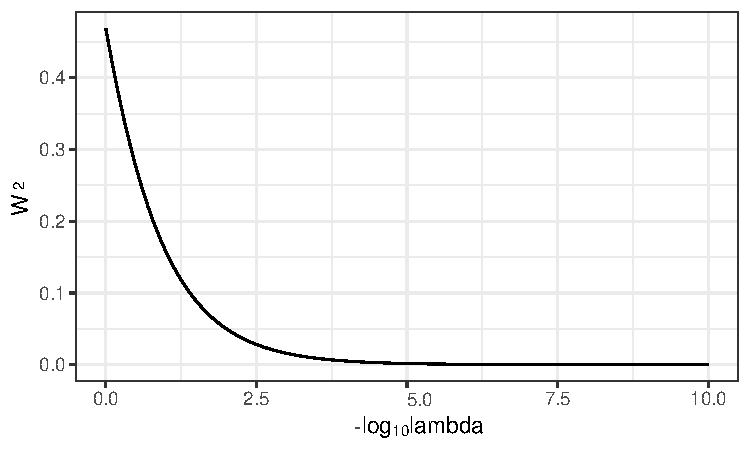
\includegraphics[width=1\textwidth]{two_normal_wass.pdf}
	\end{subfigure}
\caption{Wasserstein distance of 2nd order $W_2$ between the intrinsic and extrinsic prior for two normal random variables under sum constraint. $W_2$ declines rapidly as $\lambda$ (shown as $-\log_{10}(\lambda)$) decreases.}
\label{two_normal_wass}
\end{figure}


\subsection{\textcolor{red}{Approximation Error (Aki's proposal)}}

\aki{The convergence in total variation is too strong, so I propose something like below.}

\leo{Aki, I like your use of Feder's co-area forumula, can we get some non-asympotic result when $\lambda>m$ (away from 0)?}

\aki{A non-asymptotic result should hold as long as we put the right assumptions on $f(\theta)$. I'd think the key assumption is $\nabla f(\theta)$ to be a unit vector orthogonal to $\mc D$ whenever $\theta \in \mc D$. I don't know how to rigorously estimate the difference in the integrals over the surface $f^{-1}(0)$ and $f^{-1}(\alpha)$, however. (I can do it if $\mc D$ is a compact manifold, I think.) We may need help from an expert in geometric methods.}



\newcommand{\tilpi}{\tilde{\pi}}

We establish that the inference based on an intrinsic prior is well approximated by the one based on an extrinsic prior for sufficiently small $\lambda$. In particular, for a posterior summary of interest $g(\theta)$, we have $\mathbb{E}_{\tilpi_{\mc D, \lambda}}[g(\theta)] \to \mathbb{E}_{\pi_{\mc D}}[g(\theta)]$ as $\lambda \to 0$ provided $g(\theta)$ is continuous and integrable under the extrinsic posterior for some $\lambda < \infty$. In case the constraint takes the form $\mc D = \{f(\theta) = 0\}$ and the extrinsic posterior is given by $\tilpi_{\mc D, \lambda}(\theta) = \pi_{\mc R}(\theta) \exp(- \lambda^{-1} |f(\theta)|) \, / \, Z_\lambda$, the proof is as follows. \aki{From the proof, it appears that we also need to choose the constraint so that  $\| \nabla f \| \equiv 1$ on $\mc D$. This makes sense from geometric intuition too, I think.}

\leo{I'm not sure if $\| \nabla f \| \equiv 1$ is easy to have, for example how to scale $f(x,y)=x^3+y^3 -1$ uniformly to have $\| \nabla f \| \equiv 1$?}
\begin{proof}[Proof]
	By the co-area formula of Federer \citep{diaconis2013manifold}, we have
	\begin{equation}
	\lambda^{-1} Z_\lambda
	= \lambda^{-1} \int_{\mathbb{R}^d} \pi_{\mc R}(\theta) \exp(- \lambda^{-1} |f(\theta)|)  d \theta
	= \int_{-\infty}^{\infty}  \left[ \int_{f^{-1}(\alpha)} \frac{ g(\theta) \pi_{\mc R}(\theta) }{ \| \nabla f(\theta) \| } \mathcal{H}^{d-1}(d \theta) \right]  \lambda^{-1} \exp(- \lambda^{-1} |\alpha| ) d \alpha
	\end{equation}
	where $\mathcal{H}^{k}(d \theta)$ denotes a $k$-dimensional Hausdorff measure. Since the measure $\exp(- \lambda^{-1} |\alpha| ) d \alpha$ concentrates around $\alpha = 0$ as $\lambda \to 0$, we obtain
	\begin{equation}
	\lim_{\lambda \to 0} \lambda^{-1} Z_\lambda
	= \int_{f^{-1}(0)} \frac{ \pi_{\mc R}(\theta) }{ \| \nabla f(\theta) \| } \mathcal{H}^{d-1}(d \theta) 
	= \int_{f^{-1}(0)} \pi_{\mc D}(d \theta)
	\end{equation}
	by the assumption $\| \nabla f(\theta) \|  = 1$ and the fact that $\pi_{\mc D}(d \theta)$ coincides with the conditional density of $\pi_{\mc R}(\theta)$ on $\mc D$. Also by the co-area formula,
	\begin{equation}
	\int_{\mathbb{R}^d} g(\theta) \pi_{\mc R}(\theta) \exp(- \lambda^{-1} |f(\theta)|)  /  Z_\lambda d \theta
	= \int_{-\infty}^{\infty}  \left[ \int_{f^{-1}(\alpha)} \frac{ g(\theta) \pi_{\mc R}(\theta) }{ \| \nabla f(\theta) \| } \mathcal{H}^{d-1}(d \theta) \right]  \exp(- \lambda^{-1} |\alpha| )  /  Z_\lambda d \alpha
	\end{equation}
	Again, since the measure $\exp(- \lambda^{-1} |\alpha| ) d \alpha$ concentrates around $\alpha = 0$ as $\lambda \to 0$, we obtain
	\begin{equation}
	\lim_{\lambda \to 0} \int_{\mathbb{R}^d} g(\theta) \pi_{\mc R}(\theta) \exp(- \lambda^{-1} |f(\theta)|)  /  Z_\lambda d \theta
	= \int_{f^{-1}(0)} \frac{ g(\theta) \pi_{\mc R}(\theta) }{ \| \nabla f(\theta) \| } d \mathcal{H}^{d-1}(\theta) 
	= \frac{\int_{f^{-1}(0)} g(\theta) \pi_{\mc D}(d \theta)}{\int_{f^{-1}(0)} \pi_{\mc D}(d \theta)} \qedhere
	\end{equation}
\end{proof}


\section{Posterior Computation}

One particular appeal of the extrinsic approach is its advantage in posterior computation. As it is supported on a less restrictive space $\mc R$, one can exploit conventional sampling tools such as slice sampling, adaptive Metropolis-Hastings and Hamiltonian Monte Carlo (HMC). In this section, we focus on HMC for its easiness to use and good performance in sampling with high-dimensional parameters.

\subsection{Hamiltonian Monte Carlo for Extrinsic Posterior Sampling}

We provide a brief overview of HMC for continuous $\theta$ under extrinsic prior. Discrete extension is possible via recent work of \cite{nishimura2017discontinuous}.

In order to sample from $\theta\in\mc R \subset \mathbb R^d$, HMC introduces an auxillary momentum variable $p \sim \No(0, \mass)$. The covariance matrix $\mass$ is referred to as a \textit{mass matrix} and is typically chosen to be the identity or adapted to approximate the inverse covariance of $\theta$. HMC then sample from the joint target density $\pi(\theta, p) = \pi(\theta) \pi(p) \propto \exp (- H(\theta, p))$ where, in the case of an extrinsic posterior \eqref{extrinsic_posterior}, 

% To be clear, this is different from Riemannian HMC that requires specific accommodation and heavy computation. The algorithm we use is simply conventional HMC in Euclidean space. In this section, we study the effects of choosing $\lambda$ on efficiency of Hamiltonian dynamics.

\begin{equation}
\begin{aligned}
H(\theta, p)& = U(\theta)+K(p),\\
\text{where } & U(\theta) = -\log\left\{ L(\theta;y)\pi_{0,\mc R}(\theta) \mc{K}(\theta;\mc D) \right\},\\
& K(p) = \frac{p'\mass^{-1} p}{2}.
\end{aligned}
\end{equation}

From the current state $(\theta^{(0)},p^{(0)})$, HMC generates a proposal for Metropolis-Hastings algorithm by simulating Hamiltonian dynamics, which is defined by a differential equation:

\begin{equation}
\begin{aligned}
\label{hamiltonian}
\frac{\partial \theta ^{(t)}}{\partial t} & =\frac{\partial H(\theta, p)}{\partial p} = \mass^{-1}p,\\
\frac{\partial p^{(t)}}{\partial t}& =-\frac{\partial H(\theta, p)}{\partial \theta} = -\frac{\partial U(\theta)}{\partial \theta}.
\end{aligned}
\end{equation}

The exact solution to \eqref{hamiltonian} is typically intractable but a valid Metropolis proposal can be generated by numerically approximating \eqref{hamiltonian} with a reversible and volume-preserving  integrator \citep{neal2011mcmc}. The standard choice is the \textit{leapfrog} integrator which approximates the evolution $(\theta^{(t)},p^{(t)}) \to (\theta^{(t + \dt)},p^{(t + \dt)})$ through the following update equations:

\begin{equation}
\begin{aligned}
\label{leap-frog}
p \leftarrow p - \frac{\dt}{2} \frac{\partial U}{\partial  \theta },\quad
\theta \leftarrow  \theta  + \dt \mass^{-1}p,\quad
p \leftarrow p -  \frac{\dt}{2}  \frac{\partial U}{\partial  \theta } 
\end{aligned}
\end{equation}
Taking $L$ leapfrog steps from the current state $(\theta^{(0)},p^{(0)})$ generates a proposal $(\theta^{*},p^{*}) \approx (\theta^{(L \dt)},p^{(L \dt)})$, which is accepted with the probability 
$$1\wedge \exp  \left( - H(\theta^{*},p^{*}) + H(\theta^{(0)},p^{(0)}))\right)$$


\subsection{Support Expansion and Computing Efficiency}

While an extrinsic prior more closely approximate the constraint with a smaller $\lambda$, it turns out that computational efficiency of HMC can be negatively impacted by choosing $\lambda$ too small. In this section, we explain and quantify this phenomenon and provide a practical guidance on how to pick a reasonable value of $\lambda$.

In understanding the computational efficiency of HMC, it is useful to consider the number of leapfrog steps to be a function of $\dt$ and set $L = \lfloor \tau / \dt \rfloor$ for a fixed \textit{integration time} $\tau > 0$. In this case, the mixing rate of HMC is completely determined by $\tau$ in the limit $\dt \to 0$ \citep{betancourt17}. In practice, while a smaller stepsize $\dt$ leads to a more accurate numerical approximation of Hamiltonian dynamics and hence a higher acceptance rate, it takes a larger number of leapfrog steps and gradient evaluations to achieve good mixing. For an optimal computational efficiency of HMC, therefore, the stepsize $\dt$ should be chosen only as small as needed to achieve a reasonable acceptance rate \citep{beskos13, betancourt14}. A critical factor in determining a reasonable stepsize is the \textit{stability limit} of the leapfrog integrator \citep{neal2011mcmc}. When $\dt$ exceeds this limit, the approximation becomes unstable and the acceptance rate drops dramatically. Below the stability limit, the acceptance rate $a(\dt)$ of HMC increases to 1 quite rapidly as $\dt \to 0$ and in fact satisfies $a(\dt) = 1 - O(\dt^4)$ \citep{beskos13}.

For simplicity, the following discussions assume the mass matrix $\mass$ is taken to be the identity. Let $\hess_U(\theta)$ denote the hessian matrix of $U(\theta) = - \log \pi(\theta)$ and let $\omega_U(\theta)$ denotes the largest eigenvalue of $\hess_U(\theta)$. While analyzing stability and accuracy of an integrator is highly problem specific, the linear stability analysis and empirical evidences suggest the following; for stable approximation of Hamiltonian dynamics by the leapfrog integrator, the condition 
\begin{equation}
\label{eq:stability_condition}
\omega_U(\theta)^{1/2} \dt < 2
\end{equation} 
must hold on most regions of the parameter space $\theta$ \citep{hairer06}. When the target distribution $\pi(\theta)$ is Gaussian, we have $\omega_U^{-1} = \min_{\| u \| = 1} \textrm{var}(\langle \theta, u \rangle)$ and the stability condition \eqref{eq:stability_condition} reduces to $\epsilon < 2 \sigma_{\min}$ where $\sigma_{\min}$ is the scale of $\theta$ in the most constrained direction. (The stability analysis in this special case is also discussed in \cite{neal2011mcmc}.) In the case of an extrinsic posterior, the Hessian $\hess_U(\theta)$ is given by
\begin{equation}
\label{eq:hessian_extrinsic}
\hess_U(\theta) = -\hess_{\log \pi_{\mc R}}(\theta)  - \sum_k \lambda_k^{-1} \hess_{v_k}(\theta).
\end{equation}
The largest eigenvalue of $\hess_U(\theta)$ becomes dominated by the second term of \eqref{eq:hessian_extrinsic} and grows proportional to $\max_k \lambda_k^{-1}$ in the limit $\lambda_k \to 0$. \leo{we should add that this only applies when $\theta \not \in \mc D$}. In this asymptotic regime, according to the condition \eqref{eq:stability_condition}, the leapfrog stepsize $\dt$ needs to scale proportional to $\min_k \lambda_k^{1/2}$ for a stable approximation. Backward error analysis for the stability and approximation error similarly suggests the need for $\dt$ to scale proportional to $\min_k \lambda_k^{1/2}$ \citep{skeel2001modified}.

The purpose of our extrinsic approach is to approximate the intrinsic posterior with a sufficiently small $\lambda_k$'s. However, the above analysis reveals that, as $\lambda_k \to 0$'s, the stepsize and hence the computational cost of HMC becomes dominated by the extrinsic constraint rather than the structure of the intrinsic posterior. A reasonable choice of $\lambda_k$'s should therefore balance the computational cost of HMC and  proximity of the extrinsic posterior to the intrinsic one. Since $- \hess_{\log \pi}^{-1}$ roughly represents a local covariance structure of a density $\pi$, the square root $\omega^{-1 / 2}$ of its smallest eigenvalue can be thought of as the (local) scale of the density in its most constrained direction. In order for the second term of \eqref{eq:hessian_extrinsic} not to completely dominate the computational cost of HMC, therefore, $\min_k \lambda_k^{1/2}$ should scale proportional to the scale of the intrinsic posterior in its most constrained direction along $\mc D$.

\aki{The choice $\lambda = 10^{-3}$ cannot possibly be a universally good choice. A reasonable suggestion needs to be more like $\lambda^{1/2} \approx c \times (\text{scale of the intrinsic posterior})$. I don't know, though, how one is supposed to reasonably guess the scale of the intrinsic posterior. }

\aki{The story here does not sound very well: ``$\lambda$ needs to be small to approximate the intrinsic posterior well, but the computational costs grows like $\lambda^{-1/2}$''. It seems important to characterize that the computational cost (hopefully) grows slower than the approximation error. I conjecture that this is indeed true if $\nabla v(\theta)$ is orthogonal to $\mc D$ in which case the leading order error term is a function of the curvature of $\mc D$.}


\leo{One thing to note is that, small $\lambda_k$ is not an issue when $\theta\in \mc D$, since $\sum_k \lambda_k^{-1} \hess_{v_k}(\theta)=0$. That means if $\omega_U^{-1}$ is reasonably large for $\pi_{\mc R}(\theta)\mathbbm{1}_{\theta \in \mc D}$, we can use large $\lambda_k^{-1}$ to force $\theta\in \mc D$ for most of time. On the other hand, if $\omega_U^{-1}$ is small (without extrinsic approximation), we need smaller $\lambda_k^{-1}$ to increase $\omega_U^{-1}$, that's where the trade-off applies.}

\leo{More generally speaking, recall $\mc D= \cap_k \mc D_k$, where each $\mc D_k$ is a constrained space. It is possible that $\pi_{\mc R}(\theta)\mathbbm{1}_{\theta \in \cap A_k}$ does not have small $\omega_U^{-1}$, for a subset of constraints $\{A_k\}\subset\{\mc D_k\}$; but the overall $\pi_{\mc R}(\theta)\mathbbm{1}_{\theta \in \cap \mc D_k}$ does have this problem. Therefore, we can use large $\lambda_k^{-1}$ over the index of $\{A_k\}$ and smaller ones over $\{\mc D_k\}\setminus \{A_k\}$. The overall computational cost should be controled by $\underset{k:\{\mc D_k\}\setminus \{A_k\}}{\max} \lambda_k^{-1}$. Perhaps we can formalize on this, although I'm not sure how to incorporate Hessian with space truncation at this point.}

\aki{Another possibility is to start with $\lambda$ for which the mixing seems good enough and sequentially ``tighten'' the constraint. For example, we can do something like 1. Collect HMC samples with some fixed $\lambda$, 2. Reduce $\lambda$ and (independently) update the previous samples with a few iterations MCMC (say MALA or HMC) with this new posterior, 3. Repeat 2.}

\leo{Yes, that is one possibility. David and I talked about this a while ago. We didn't go in this direction because we want to keep the algorithm as simple as possible, provided the approximation error is reasonably bounded, then we can suggest projection or adaptive algorithm as follow-up remedy. I think a non-asymptotic bound on approximation error and some numeric Wasserstein/ TV distances on the examples below should suffice; but I'm open to new algorithm if really necessary.}





\section{Simulated Examples and Application}

We now use examples to illustrate the properties of extrisinc priors and their utility in common scenarios.

\subsection{Simulations}

{\bf Example 2: Linear Regression Under Inequality Constraint}

When the support on constrained space $\mc D$ has $w_\pi$ away from $0$, one can use extrinsic prior with almost no support expansion. This applies a large class of inequality constraints that has wide support. For example, consider a linearly constrained regression model:

$$y_i \sim \No (x_i \theta, \sigma^2) \text{ for } i=1,\ldots n, \quad\text{ with } A\theta \le c$$
where parameter $\theta$ is a $p$-dimensional vector; the constraint parameters $A$, a $d\times p$ matrix, and $c$, a $d$-dimensional vector, are both given. The inequalities form one or multiple polyhedrons in $\mathbb R^p$, with $\mc D$ as the interior or exterior space.

We consider simple bivariate case $\theta \in (0,1)^2$ subject to $\theta_1+\theta_2\le 1$, making $\mc D$ a triangle. To simulate data, we use $\sigma^2=0.1^2$, $x_i\sim \No([0,0]',I)$ for $i=1,\ldots,n$. We then generate two datasets using different values of $\theta$ and $n$. In the first experiment, we use $\theta=[0.3,0.3]'$ with $n=10$, so that the posterior has wide spread and centered in the interior of $\mc D$; in the second experiment, we use $\theta=[0.7,0.3]'$ with $n=10^4$ so that the posterior is concentrated on the boundary. In both cases, we assign weakly informative prior for $\theta\sim \No([0.5, 0.5]',I10^2)$ and inverse-Gamma prior $\sigma^2\sim \text{IG}(2,1)$.

We use $\mc K(\theta)=\exp( - \frac{v(\theta)}{\lambda})$ with $v(\theta)=|\theta_1+\theta_2-1|_{+}$ in the extrinsic prior. We choose $\lambda=10^{-8}$ leading to almost no support expansion. We collect $10,000$ posterior samples efficiently via HMC. The Markov chain mixes rapidly , generating $10,000$ effective sample size in both experiments. Figure~\ref{linear_inequality} plots the posterior sample and its contour. There is no posterior that fall outside $\mc D$, thanks to small $\lambda$.

\begin{figure}[H]
   \begin{subfigure}[b]{0.45\textwidth}
    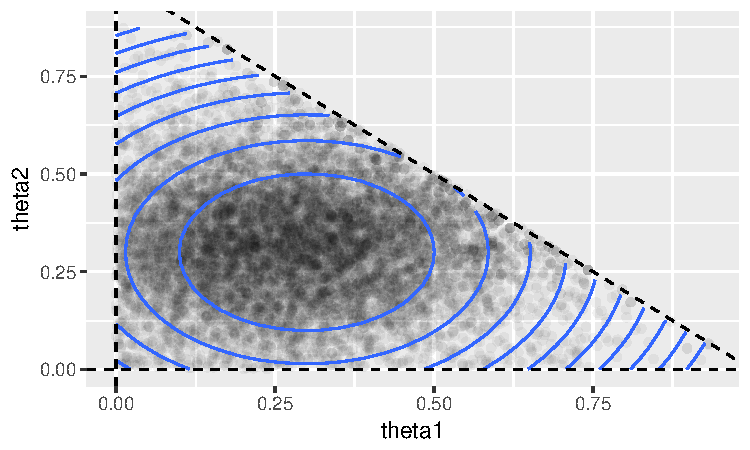
\includegraphics[width=1\textwidth]{linear_inequal_1}
    \caption{$n=10$ with true $\theta=[0.3,0.3]'$}
	\end{subfigure}
    \begin{subfigure}[b]{0.45\textwidth}
     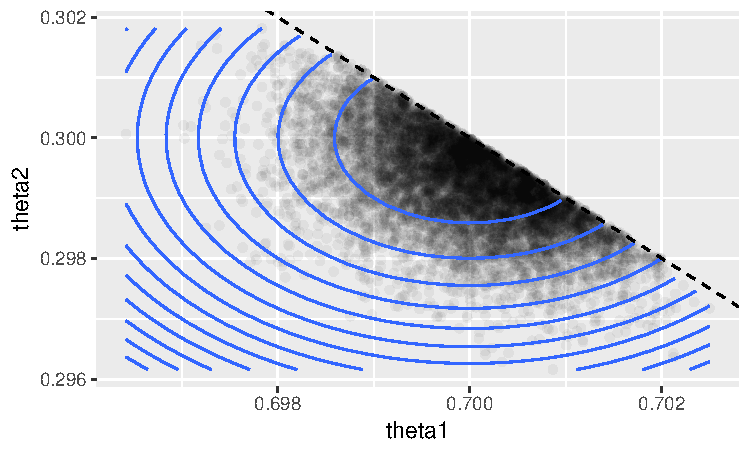
\includegraphics[width=1\textwidth]{linear_inequal_2}
     \caption{$n=10^4$ with true $\theta=[0.7,0.3]'$}
     	\end{subfigure}
\caption{Extrinsic posterior distribution of the normal mean $\theta$, with approximation to constraint $\theta_1+\theta_2\le 1$. Posterior is either loosely distributed near the center (panel (a)) or concentrated on the boundary (panel (b)) of the region. The extrinsic posterior has no samples outside of the region due to almost no relaxation.}
\label{linear_inequality}
\end{figure}

{\bf Example 3: Unit Circle}

If the constrained support in $\mc D$ has a minimum support width $w_\pi$ close to $0$, it limits the stability bound and computing efficiency in continuous HMC. In this example, we consider $\mc D$ is a two-dimensional unit cirlce $\{(\theta_1,\theta_2):\theta_1^2+\theta_2^2=1\}$ (alternatively, $V(2,1)$, a $(2,1)$--Stiefel manifold). In this space, $w_\pi =0$ hence support expansion is necessary.

Let data $y_i\in \mathbb{R}^2$ for $i=1,\ldots,n$  be noisy realization from one point on unit circle:

$$y_i\sim \No(\theta, I_2\sigma^2),\text{ with } \theta'\theta=1,$$
where $\theta \in \mc D$ is assigned a von Mises--Fisher prior $\pi_{0,\mc D}(\theta) \propto \exp(F'\theta_i)$.

 To generate data, we use $\theta= (\sqrt 3/2, 1/2)$, $\sigma^2=0.5^2$ and small $n=5$, in order to induce widely spread-out posterior $\theta$ on the manifold. We then use $F=(1,1)$ to induce a weakly informative prior for $\theta$ and an inverse-Gamma prior $\text{IG}(2,1)$ for $\sigma^2$ . To assign extrinsic prior, we use $v(\theta)=|\theta'\theta -1|$ as the distance to circle and extrinsic prior $\tilde\pi_{0,\mc D}(\theta)= \exp(F'\theta_i) \exp(-\frac{|\theta'\theta -1|}{\lambda})$.

We test $\lambda = 0.001$, $0.0001$ and $0.00001$ in three experiments. We run each algorithm for $20,000$ steps, with first $10,000$ discarded. To compare the computing efficiency, we restrict the maximum leap-frog steps $L$ to be $100$ and visualize how much space each algorithm can explore within one HMC iteration. Figure~\ref{unit_circle}(a) plots the path of $L=100$ leap-frog steps. Larger $\lambda$ leads to wider support expansion and larger stability bound $\epsilon_{max}$. This makes $\theta^{(\epsilon L)}$  much less correlated with $\theta^{(0)}$ at each iteration, measured by autocorrelation (ACF) based on the posterior sample of $\theta_1$ (Figure~\ref{unit_circle}(b)). Even though we use somewhat small $\lambda$, the posterior distance $v(\theta)$ is small for all three settings (Figure~\ref{unit_circle}(c)), with smaller $\lambda$ associated with smaller $v(\theta)$ but lower computing efficiency.

\begin{figure}[H]
\centering
   \begin{subfigure}[b]{0.8\textwidth}
    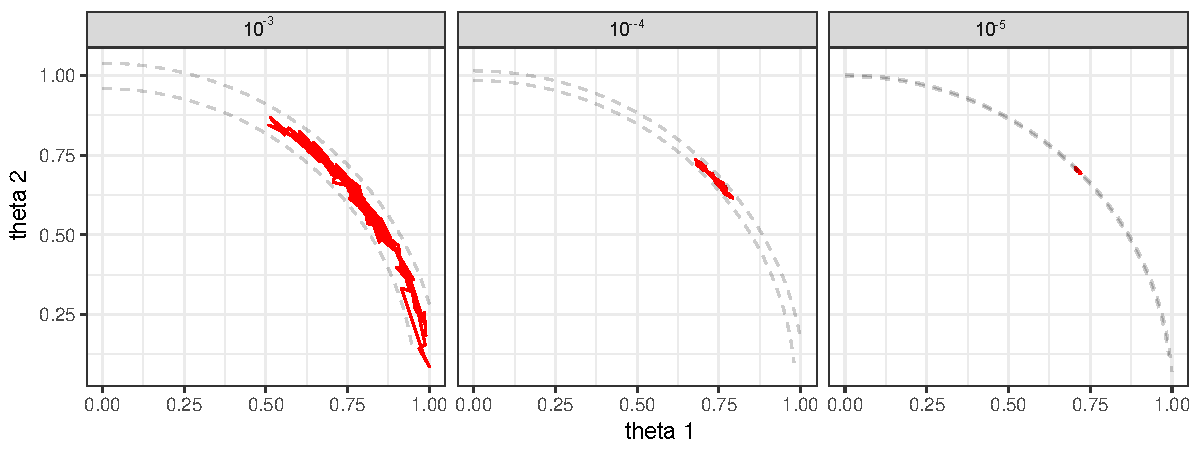
\includegraphics[width=1\textwidth]{unit_circle_100steps}
    \caption{Path of 100 itegrator steps in one HMC iteraton}
	\end{subfigure}
    \begin{subfigure}[b]{0.8\textwidth}
     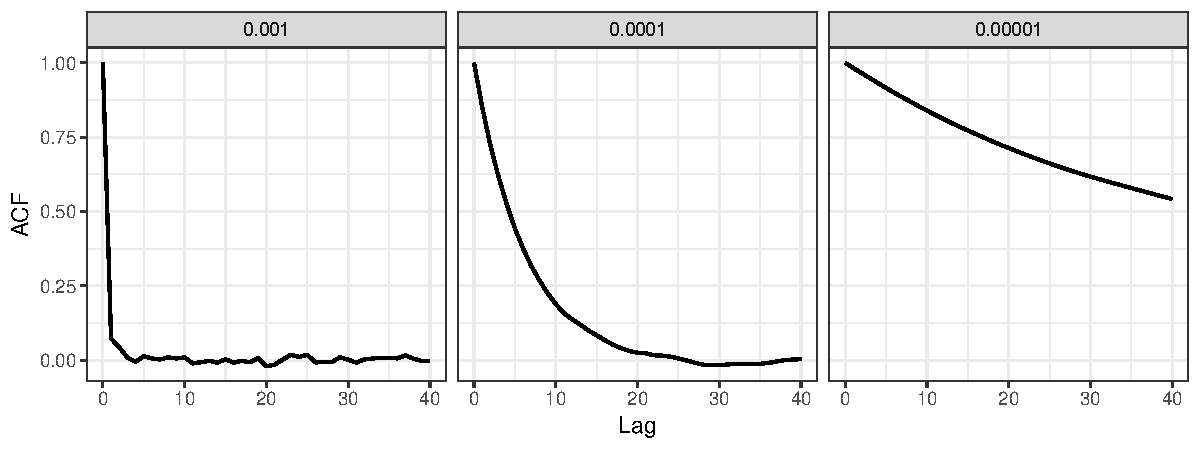
\includegraphics[width=1\textwidth]{unit_circle_acf}
     \caption{Autocorrelation of $\theta_1$}
     	\end{subfigure}
    \begin{subfigure}[b]{0.8\textwidth}
    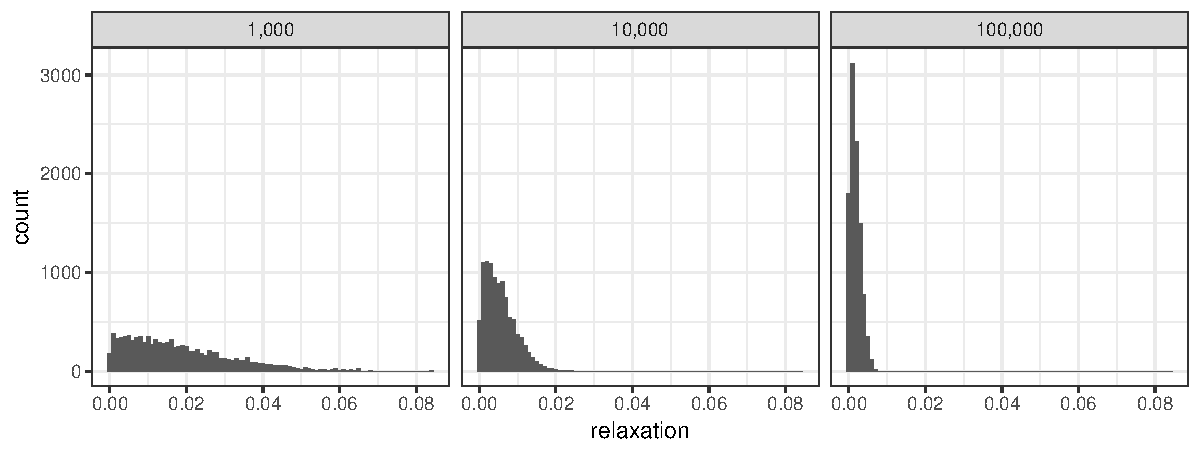
\includegraphics[width=1\textwidth]{unit_circle_violation}
         \caption{Posterior distribution of  $|\theta'\theta-1|$}
    	\end{subfigure}
\caption{HMC Sampling on a unit circle, using extrinc prior with $\mc K(\theta)=\exp(-\frac{|\theta'\theta -1|}{\lambda})$, with $\lambda=0.001$, $0.0001$ and $0.00001$. Panel (a) shows the larger relaxation in the narrowest direction of support (orthogonal vector to the circle) can result in more efficient space exploration within $100$ leap-frog steps; panel (b) shows the autocorrelation of the posterior sample; panel (c) shows the posterior distribution of the distance to the constraint.}
\label{unit_circle}
\end{figure}

\subsection{Applications}

In statistical modeling, it is common to encounter parameters or latent variables that are non-identifiable. Imposing constraints can often solve or reduce such issue, although they tend to make the computation difficult. We now illustrate utility of extrinsic prior for two applications.  

{\bf Example 3: Ordered Dirichlet Prior}

We first consider ordered simplex in finite mixture model. A $(J-1)$--simplex is a vector $w=\{w_1,\ldots w_J\}$ with $1> w_1 \ge \ldots \ge w_J > 0$ and $\sum_{j=1}^J w_j=1$.

For probablity simplex, standard practice assigns Dirichlet prior $Dir(\alpha)$, with $
\pi_{0, \mc D}(w) = \prod_{j=1}^J w_j^{\alpha-1} \1_{\sum_{j=1}^J w_j=1}$. However, this does not accomodate ordering; therefore, the index $j$ is exchangeable and permutating $j$'s does not change the density. This commonly leads to label-switching problem in mixture model estimation (reviewed in \cite{jasra2005markov}).

Imposing order constraint yields an ordered Dirichlet prior:

 \begin{equation}
\begin{aligned}
\label{ordered_dp_prior}
\pi_{0, \mc D}(w_1,\ldots w_J) \propto \prod_{j=1}^J w_j^{\alpha-1} \cdot \1_{\sum_{j=1}^J w_j=1} \cdot  \prod_{j=1}^{J-1}\1_{w_j \ge w_{j+1}}.
\end{aligned}
\end{equation}
where $w_j\in (0,1)$ for $j=1,\ldots,J$. The ordered Dirichlet prior can be approximated by extrinsic prior:

 \begin{equation*}
\begin{aligned}
\tilde\pi_{0, \mc D}(w_1,\ldots w_J)  \propto \prod_{j=1}^J w_j^{\alpha-1} \cdot  \exp ( -  \frac{ \sum_{j=1}^J ( w_{j+1} - w_j )_+}{\lambda_1})
 \exp ( -  \frac{|{\sum_{j=1}^J w_j - 1}|}{\lambda_2})
\end{aligned}
\end{equation*}

We now adopt this simplex distribution in a normal mixture model with mixture means and common variance, for data $y_i\in \bb R^d$ indexed by $i=1,\ldots,n$:

\begin{equation*}
\begin{aligned}
y_i &\stackrel{indep}{\sim} \No(\mu_i,\Sigma),\qquad
\mu_i &\stackrel{iid}{\sim} G,\qquad
G(.) & = \sum_{j=1}^{J} w_j \delta_{\mu_j}(.),
\end{aligned}
\end{equation*}
where $\delta_{b}(a)=1$ if $a=b$ and $0$ otherwise.

We generate $n=100$ samples from $3$ components with true $\{w_1,w_2,w_3\}=\{0.6,0.3,0.1\}$ and two-dimensional means $\{\mu_1,\mu_2,\mu_3\} = \{[1,5], [3,3], [3,5]\}$ with identity covariance $\Sigma = I_2$. We assign weakly informative priors $\No(0,10 I_2)$ for each $\mu_j$ and inverse Gamma prior for the digonal element in $\Sigma=\diag(\sigma_1^2,\sigma_2^2)$ with $\sigma^2_1, \sigma^2_2\sim IG(2,1)$. We use $\lambda_1 = 10^{-6}$ to induce almost no relaxation on the ordering and $\lambda_2 = 10^{-3}$ to allow efficient mixing in embedding a simplex in $(0,1)^J$. To illustrate the benefit of ordered Dirichlet, we also test Gibbs sampling and extrinsic prior method on canonical Dirichlet prior without order constraint.

Figure~\ref{dirichlet}(a) shows the contour of true posterior density of $\mu_j$'s. The small component sample size leads to large overlap among the posterior of $\mu_j$'s, generting in significant label-switching in both Gibbs and HMC under canonical Dirichlet prior. Figure~\ref{dirichlet}(b,c,d) show the traceplot of $w$. Ordered Dirchlet has clearly better convergence due to ordering.


\begin{figure}[H]
\begin{center}
   \begin{subfigure}[b]{0.3\textwidth}
    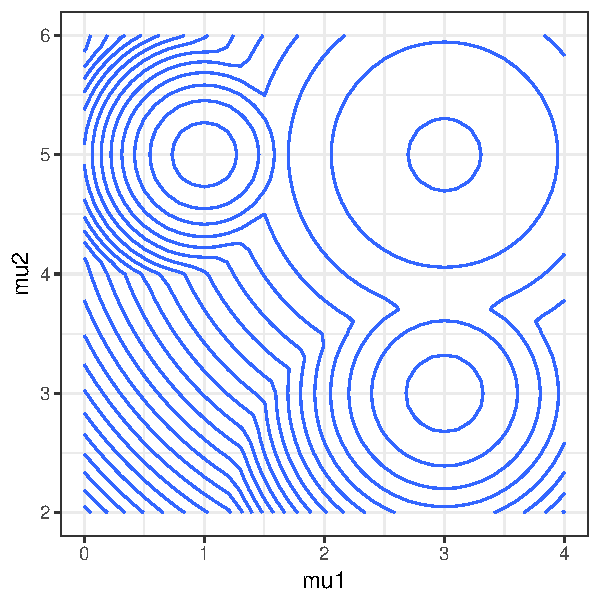
\includegraphics[width=1\textwidth]{fmm_mu_contour.pdf}
    \caption{Posterior density of the component means.}
    \end{subfigure}
    \end{center}
    \centering
   \begin{subfigure}[b]{0.32\textwidth}
    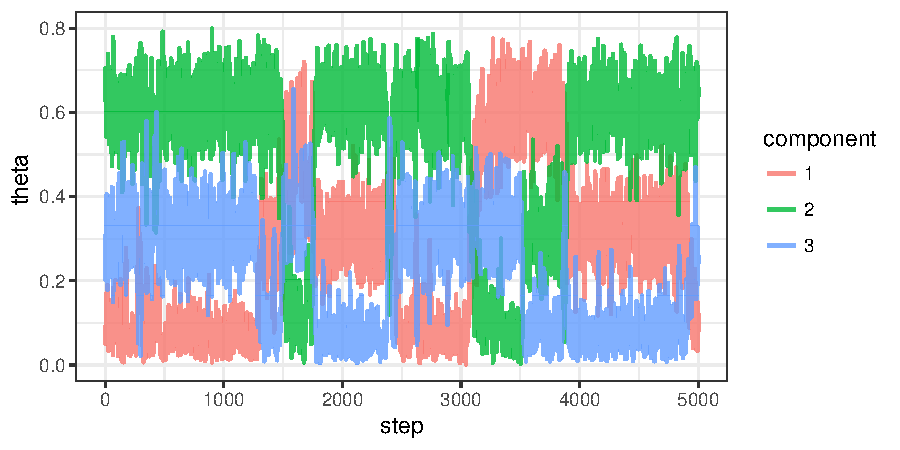
\includegraphics[width=1\textwidth]{fmm_w_gibbs.pdf}
    \caption{Gibbs sampling under canonical Dirichlet}
    \end{subfigure}
       \begin{subfigure}[b]{0.32\textwidth}
  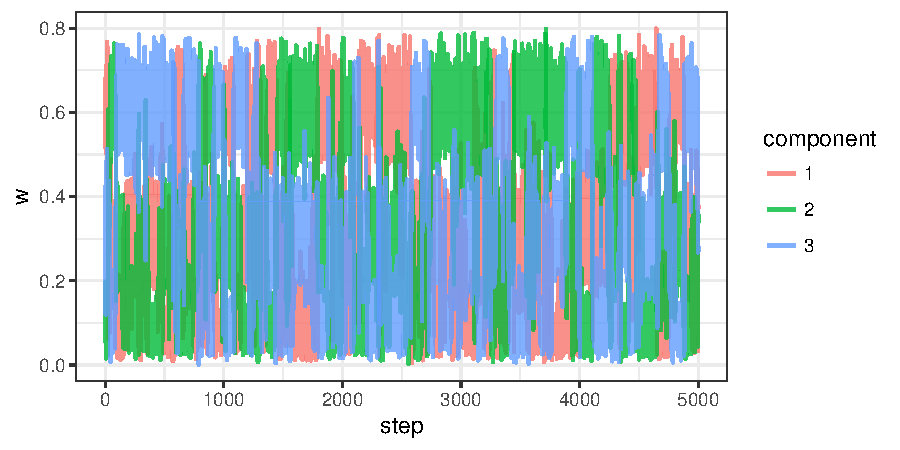
\includegraphics[width=1\textwidth]{fmm_w_hmc_unordered.pdf}
    \caption{HMC sampling under canonical Dirichlet, with extrinsic prior}
      \end{subfigure}
       \begin{subfigure}[b]{0.32\textwidth}
 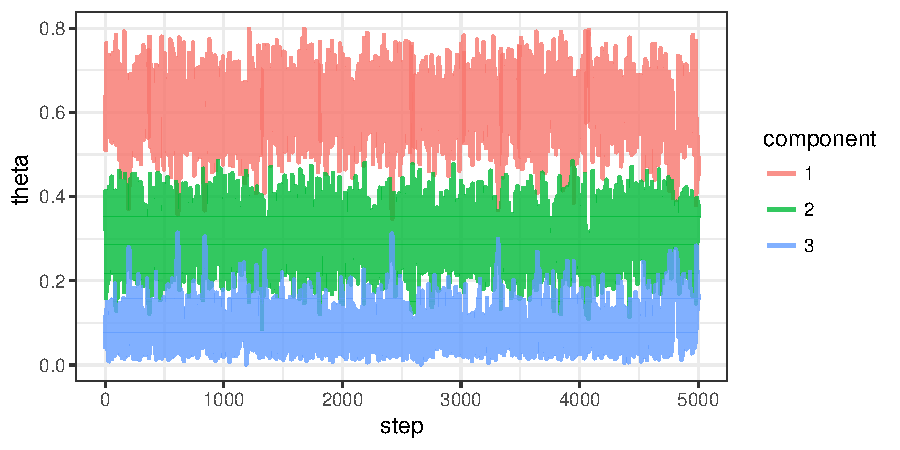
\includegraphics[width=1\textwidth]{fmm_w_hmc.pdf}
     \caption{HMC sampling under ordered Dirichlet, with extrinsic prior}
     \end{subfigure}
\caption{Contour of the posterior density of component means and traceplot of the posterior sample for the component weights $w$, in a 3-component normal mixture model. Panel (a) shows that there is significant overlap among component means $\mu_j$'s, creating label-switching issues in both Gibbs sampling (b) and HMC using canonical prior (c). The ordered Dirichlet prior significantly reducing label-switching (d).}
\label{dirichlet}
\end{figure}


{\bf Example 4: Orthonormal Tensor Factorization of Multiple Undirected Networks}

We now consider a real data application in brain network analysis. The brain connectivity structures are obtained in the data set KKI-42 (Landman et al. 2011), which consists of $21$ healthy subjects without any history of neurological disease. Each subject has two brain network observations from scan--rescan, yielding a total of n = 42. Each observation is a $V\times V$ symmetric network $A_i$, recorded as adjacency matrix $A_i$ for $i=1,\ldots,n$. For the $i$th matrix $A_i$, $A_{i,k,l} \in \{0,1\}$ is element on the $k$th row and $l$th column of $A_i$, with $A_{i,k,l}=1$ indicating there is an connection betwen $k$th and $l$th region, $A_{i,k,l}=0$ if there is no connection. The regions are constructed via the Desikan et al. (2006) atlas, for a total of V = 68 nodes.

The ambient dimension of observation is $V(V-1)/2=2,278$, which is significantly larger than sample size $n=40$. They potentially contain observational error in recording connectivity, and the  diagonal in each $A_{i}$ is missing due to the lack of interpretable self-connectivity. These facts motivate a probabilitic low-rank model approach. We consider a symmetric tensor decomposition model:

\begin{equation*}
\begin{aligned}
& A_{i,k,l} \sim \text{Bern}( \frac{1}{1+ \exp(-\psi_{i,k,l}- Z_{k,l})})\\
& \psi_{i,k,l} = \sum_{r_1=1}^{d_1}\sum_{r_2=1}^{d_2} D_{r_1,r_2} W_{i,r_2} U_{k,r_1} U_{l,r_1}  \\
\end{aligned}
\end{equation*}
for $k>l$, $k=2,\ldots, V$, $i=1,\ldots,n$; $U$ is $V\times d_1$ matrix, $W$ is $n\times d_2$ matrix; $D$ is a $d_1\times d_2$ array. The  $V\times V$ matrix $Z$ is almost unstructural except symmetric $Z_{k,l}=Z_{l,k}$, which is commonly used to induce low-rank in the decomposition \citep{durante2016nonparametric}.


This model is a special Tucker decomposition with a sparse core tensor, whose diagonal plane is equal to $D$ and $0$ for other elements. The Tucker decomposition is more flexible than another routinely used decomposition, namely parallel factor analysis (PARAFAC). The PARAFAC assumes all ranks are equal and the core tensor $D$ only has non-zero value when all its sub-indices are equal. In this case, PARAFAC would assume $d_1=d_2$. The additional flexibility in the Tucker is appealing, as one would utilize the varying rank over different sub-direction (mode) of the tensor. On the other hand, a completely unconstrained Tucker decomposition is not identifiable in the matrices and core tensor, due scaling. For example, one can multiply a $d_1\times d_1$ non-zero diagonal matrix $R$, to $U$ and obtain $U^*=UR$ obtain $D=R^{-2}D_{r_1,.,}$. This leaves the likelihood unchanged, creating identifiability issue. 

Therefore, we consider applying some constraint on the Tucker decomposition, while still maintaining its varying rank property over different modes. Motivated by high-order singular value decomposition, we impose orthonormality constraints $U'U=I_{d_1}$ and $W'W=I_{d_2}$.

We assign normal prior for $U_{k,r_2}\sim \No(0,\phi_{1})$, $W_{i,r_1}\sim \No(0,\phi_2)$, $Z_{k,l}\sim \No(0,\phi_3)$, $D_{r_1,r_2}\sim No(0, \phi_{4,r_1,r_2})$ for all $i,k,l,r_1,r_2$, and inverse-Gamma prior $\phi_1,\phi_2,\phi_3\stackrel{indep}{\sim} \text{IG}(2,1)$, $\phi_{4,r_1,r_2}= \tau_{r_1}\tau_{r_2}$, with $\tau_{r_1},\tau_{r_2}\stackrel{indep}{\sim} \text{IG}(2,1)$ for all $r_1,r_2$.

%we assign multiplicative inverse gamma distribution \citep{bhattacharya2011sparse} $\phi_{4,r_1,r_2}= \prod_{m_1=1}^{r_1} \nu_{1,m_1} \prod_{m_2=1}^{r_2}  \nu_{2,m_2}$ with $\nu_{1,1},\nu_{2,1} \stackrel{indep}{\sim} \text{IG}(a_1,1)$ and $\nu_{1,m},\nu_{2,m}\stackrel{indep}{\sim} \text{IG}(a_2,1)$ for $m\ge 2$. This induces increasing concentration toward zero as $r_1,r_2$ increase, allowing adaptive choosing of latent dimensions. We set $a_1=a_2=5$ in this application.

To allow estimation for model with orthonormality constraint, we use extrinsic prior with $\mc K(\theta) = \exp( - \frac{(U'U-I_{d_1})^2 + (W'W-I_{d_2})^2  }{\lambda})$ and set $\lambda=10^{-3}$. To compare, we also test with the same model configuration without the orthonormality constraint. We run both models for $10,000$ steps and discard the first $5,000$ steps. Figure~\ref{tucker} plots the traceplot and autocorrelation for matrix $U$. Unconstrained model has severe convergence issue due to the non-identifiability, while constrained model converges and show low autocorrelation for all the parameters.

\begin{figure}[H]
   \begin{subfigure}[b]{1\textwidth}
    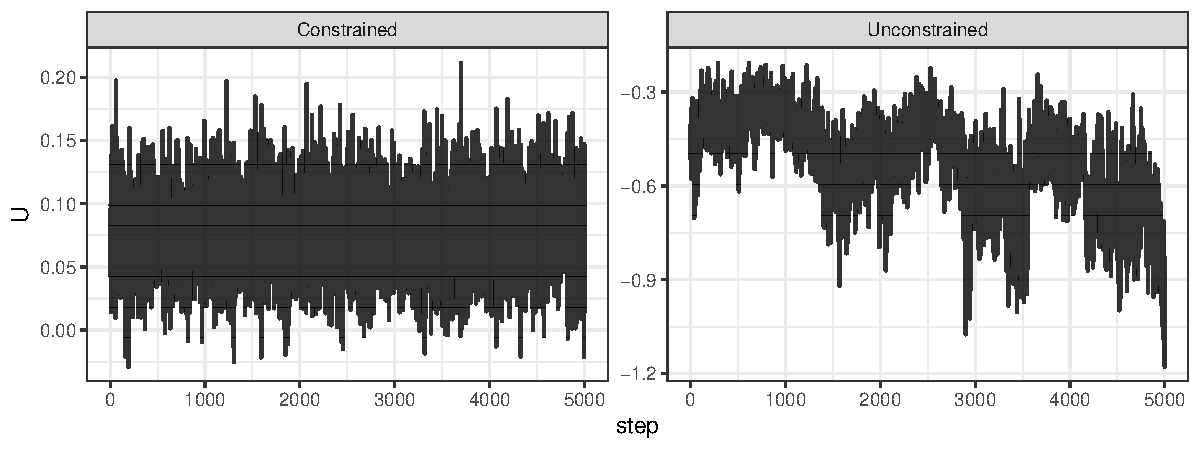
\includegraphics[width=1\textwidth]{tucker_traceplot.pdf}
    \caption{Traceplot of $U_{1,1}$.}
    \end{subfigure}
    \begin{subfigure}[b]{1\textwidth}
    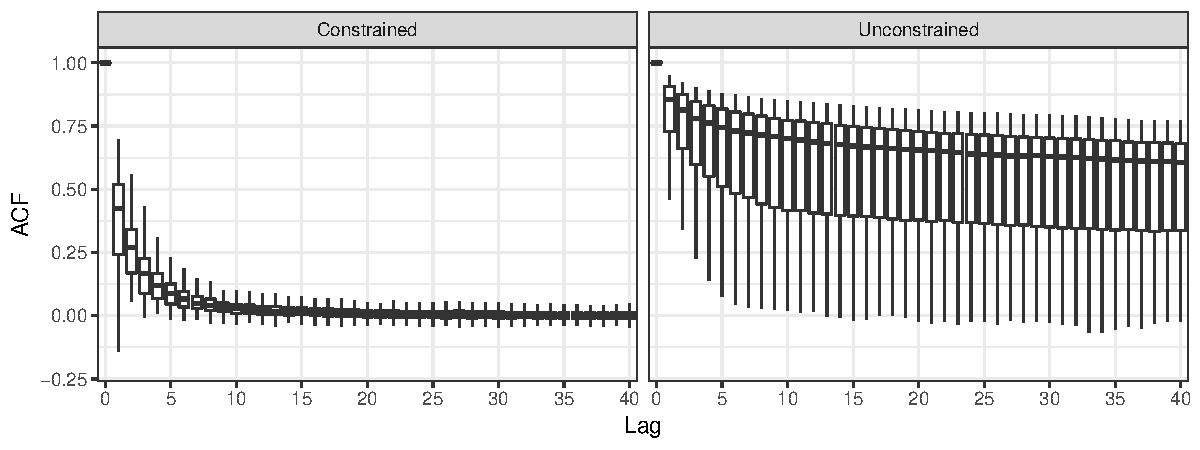
\includegraphics[width=1\textwidth]{tucker_acf.pdf}
    \caption{ACF of all elements in $U$}
    \end{subfigure}
\caption{Orthonormality constraint in the tensor decomposition modelallows convergence and rapid mixing on the factor matrix (left column); whereas unconstrained model does not converge due to free scaling.}
\label{tucker}
\end{figure}

\section{Discussion}



\bibliography{reference}
\bibliographystyle{apalike} %TODO: change back to chicago.

\end{document}
